% !TeX program = xelatex
%% Báo cáo ViCivil-TKG - bản PDF chuyên nghiệp
%% Biên dịch: xelatex report.tex (2 lần) ; font: Arial/Consolas (hỗ trợ đầy đủ dấu tiếng Việt)
\documentclass[11pt,a4paper]{article}

\usepackage{fontspec}
\setmainfont{Arial}
\setsansfont{Arial}
\setmonofont{Consolas}[Scale=0.92]
\usepackage{polyglossia}
\setdefaultlanguage{vietnamese}

\usepackage[top=2.4cm,bottom=2.2cm,left=2.4cm,right=2.4cm]{geometry}
\usepackage{xcolor}
\usepackage{graphicx}
\usepackage{booktabs}
\usepackage{array}
\usepackage{longtable}
\usepackage{caption}
\usepackage{enumitem}
\usepackage{fancyhdr}
\usepackage{titlesec}
\usepackage[hidelinks]{hyperref}
\usepackage{amsmath}
\usepackage{microtype}
\usepackage[most]{tcolorbox}

\graphicspath{{figures/}}

\definecolor{gold}{HTML}{B8860B}
\definecolor{ink}{HTML}{1F3A52}
\definecolor{muted}{HTML}{5A6570}
\definecolor{rule}{HTML}{D8DEE6}
\definecolor{panel}{HTML}{F4F6F8}

\captionsetup{font=small,labelfont={bf,color=ink},labelsep=period,skip=6pt}
\captionsetup[table]{position=top}

\titleformat{\section}{\Large\bfseries\color{ink}}{\thesection}{0.7em}{}
\titleformat{\subsection}{\large\bfseries\color{ink}}{\thesubsection}{0.6em}{}
\titlespacing*{\section}{0pt}{18pt}{8pt}
\titlespacing*{\subsection}{0pt}{12pt}{6pt}

\pagestyle{fancy}
\fancyhf{}
\setlength{\headheight}{15pt}
\fancyhead[L]{\footnotesize\color{muted}ViCivil-TKG --- Báo cáo kỹ thuật v1.5.4}
\fancyhead[R]{\footnotesize\color{muted}\thepage}
\renewcommand{\headrulewidth}{0.4pt}
\renewcommand{\headrule}{\hbox to\headwidth{\color{rule}\leaders\hrule height \headrulewidth\hfill}}

\setlist[itemize]{leftmargin=1.3em,itemsep=2pt,topsep=3pt}
\setlist[enumerate]{leftmargin=1.6em,itemsep=2pt,topsep=3pt}
\renewcommand{\arraystretch}{1.22}

\newtcolorbox{keybox}[1][]{colback=panel,colframe=rule,boxrule=0.5pt,arc=2pt,
  left=6pt,right=6pt,top=5pt,bottom=5pt,#1}
\newcommand{\src}[1]{\textcolor{muted}{\footnotesize Nguồn: #1}}

\begin{document}

% ============================== TRANG BÌA ==============================
\begin{titlepage}
\centering
\vspace*{1.2cm}
{\color{gold}\rule{\linewidth}{1.2pt}}\\[6pt]
{\footnotesize\color{muted}\MakeUppercase{Báo cáo kỹ thuật --- phiên bản dữ liệu v1.5.4}}\\[10pt]
{\Huge\bfseries\color{ink} ViCivil-TKG\par}
\vspace{6pt}
{\Large Khung tri thức thời gian của luật dân sự Việt Nam\par}
\vspace{4pt}
{\large\color{gold} Dữ liệu mở, đồ thị có chiều thời gian và trình xem mở}\par
\vspace{1.2cm}
{\color{gold}\rule{0.55\linewidth}{0.8pt}}\\[14pt]

\begin{minipage}{0.86\linewidth}\centering\small
\begin{tabular}{@{}ll@{}}
\toprule
Văn bản luật trong kho & 17 văn bản (kèm 16 văn bản sửa đổi bên ngoài) \\
Đoạn văn bản cắt nhỏ (chunk) & 11.267 \\
Văn bản trong đồ thị / quan hệ & 33 / 21 \\
Câu hỏi kiểm tra & 281 \\
Phần mềm dùng & 4 thư viện mở, không CDN, không cần cài đặt \\
\bottomrule
\end{tabular}
\end{minipage}

\vfill
\begin{minipage}{0.86\linewidth}\small
\begin{tabular}{@{}ll@{}}
\toprule
Kho mã & \texttt{github.com/ntd25022006q/vicivil-tkg} \\
Gương phát hành & \texttt{huggingface.co/datasets/datbazuka2502/vicivil-tkg} \\
Trang xem trực tuyến & \texttt{ntd25022006q.github.io/vicivil-tkg/graph/explorer.html} \\
Ngày lập & 20/10/2026 \\
\bottomrule
\end{tabular}
\end{minipage}

\vspace{1cm}
{\footnotesize\color{muted}
Mọi hình trong báo cáo này là ảnh chụp từ trang đang chạy, ảnh chụp nguyên văn từ tệp trong kho,
hoặc sơ đồ vẽ bằng công cụ Mermaid (mã nguồn nằm trong kho). Mọi con số đều lấy từ tệp dữ liệu
và có thể mở kiểm tra trực tiếp.}
\end{titlepage}

% ============================== TÓM TẮT ==============================
\section*{Tóm tắt}
\addcontentsline{toc}{section}{Tóm tắt}

Luật dân sự Việt Nam không có một bản duy nhất: Bộ luật Dân sự 1995 bị thay bằng bản 2005,
bản 2005 bị thay bằng bản 2015, và các luật chuyên ngành hôn nhân gia đình, tố tụng, thừa tụng
liên tục sửa đổi lẫn nhau. Khi tra cứu, câu hỏi đầu tiên không phải ``điều khoản nào nói về
điều này'' mà là \emph{vào thời điểm đó, điều khoản nào còn có hiệu lực}.

Công trình này dựng một bộ dữ liệu trả lời được câu hỏi đó, gồm bốn phần: kho 11.267 đoạn
văn bản đã cắt nhỏ và gán mã ổn định; đồ thị tri thức 33 văn bản với 21 quan hệ có mốc thời gian;
bộ 281 câu hỏi để đo chất lượng truy hồi; và một trang xem để kiểm chứng bằng mắt. Trang xem chạy
được hoàn toàn khi mất mạng, không cần cài đặt.

Kết quả đo trên 281 câu hỏi có đáp án: tỉ lệ tìm đúng trong 1 lần là 0,452; trong 3 lần là 0,658;
trong 5 lần là 0,726; trong 10 lần là 0,794; độ tin cậy tổng hợp 0,569. Trên 245 câu đã được tác
giả xác minh, tỉ lệ tìm đúng trong 1 lần là 0,502.

\tableofcontents
\clearpage

% ============================== 1 ==============================
\section{Đặt vấn đề}

Luật dân sự Việt Nam có hiệu lực theo thời gian. Mỗi văn bản có một khoảng thời gian
``từ ngày nào đến ngày nào có hiệu lực'', và các văn bản nối với nhau bằng quan hệ thay thế
hoặc sửa đổi. Một câu hỏi tra cứu pháp lý thường mang theo thời điểm: ``tại thời điểm T, quy định
này còn hiệu lực không?''. Muốn trả lời, người ta cần dữ liệu ở dạng có chiều thời gian, chứ
không phải một danh sách văn bản phẳng.

Báo cáo này mô tả bộ dữ liệu ViCivil-TKG: cách xây dựng, cách kiểm chứng, kết quả đo, và
những điểm còn thiếu cùng đề xuất bổ sung.

\begin{keybox}
\textbf{Quy ước dùng trong báo cáo.} Văn bản luật được gọi tắt là \emph{luật}. Đoạn văn bản
nhỏ dùng để tra cứu được gọi là \emph{chunk} và mang một mã duy nhất. Số liệu trong báo cáo luôn
lấy từ tệp trong kho và có thể mở kiểm tra.
\end{keybox}

% ============================== 2 ==============================
\section{Dữ liệu dùng và quy trình từ A đến Z}

\subsection{Nguồn}

Sáu tệp PDF chính thức được lấy từ công báo: Bộ luật Dân sự 1995, 2005, 2015; Luật Hôn nhân và
Gia đình 2014; Luật Tố tụng 2017; Nghị định 152/2026. Mỗi tệp lưu kèm đường dẫn nguồn, loại nguồn
(\textit{mirror}, \textit{official}, \textit{semi-official}) và ngày lấy trong
\texttt{provenance/law\_sources.json}.

\subsection{Quy trình}

\begin{figure}[htbp]
\centering
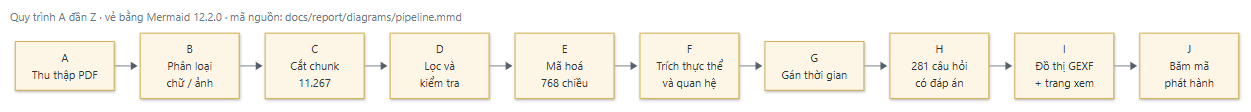
\includegraphics[width=\textwidth]{fig01_quy-trinh.png}
\caption{Dải nhìn tổng quan quy trình từ A đến Z. Vẽ bằng công cụ Mermaid; mã nguồn sơ đồ
nằm trong kho tại \texttt{docs/report/diagrams/pipeline.mmd}. Chi tiết từng bước và tệp đầu ra
ở Bảng \ref{tab:steps}.}
\label{fig:pipeline}
\end{figure}

\begin{table}[htbp]
\centering\small
\caption{Các bước xây dựng và tệp chứng minh cho từng bước.}
\label{tab:steps}
\begin{tabular}{@{}cp{6.3cm}p{6.3cm}r@{}}
\toprule
\textbf{Bước} & \textbf{Nội dung} & \textbf{Tệp đầu ra} & \textbf{Số lượng} \\
\midrule
A & Lấy PDF công báo, lưu nguồn và ngày lấy & \texttt{provenance/law\_sources.json} & 6 tệp \\
B & Phân biệt PDF chữ và PDF ảnh; ảnh vào hàng chờ OCR & \texttt{sources\_raw/} & --- \\
C & Cắt nhỏ theo Điều --- Khoản --- Điểm, gán mã & \texttt{data/civil\_chunks.jsonl} & 11.267 chunk \\
D & Lọc luật dân sự, chặn chunk rỗng / trùng mã / luật mồ côi & \texttt{provenance/law\_audit.json} & 0 lỗi \\
E & Mã hoá mỗi chunk thành 768 con số & \texttt{index/vdb\_chunks.json} & 11.267 vector \\
F & Rút thực thể và quan hệ giữa các chunk & \texttt{index/kv\_store\_*.json} & 3 kho \\
G & Gán khoảng hiệu lực cho từng luật, dựng chuỗi kế thừa & \texttt{provenance/temporal\_graph.json} & 33 luật \\
H & Làm câu hỏi có đáp án và chấm điểm hệ thống & \texttt{benchmark/law\_eval\_v12.json} & 281 câu \\
I & Xuất đồ thị GEXF và dựng trang xem & \texttt{docs/graph/} & 1 trang \\
J & Băm mã SHA-256, đồng bộ hai gương, đóng thẻ phiên bản & \texttt{SHA256SUMS} & 62 tệp \\
\bottomrule
\end{tabular}
\end{table}

Mỗi bước đều có một tệp đầu ra kiểm chứng được:

% ============================== 3 ==============================
\section{Chia nhỏ văn bản và gán mã}

Chunk là đơn vị trích dẫn nhỏ nhất mà luật dân sự dùng để quy định nghĩa vụ, tức là
Điều --- Khoản --- Điểm. Mỗi chunk mang một mã ổn định, ví dụ \texttt{BLDS2015|Dieu27|Khoan1|Diema}.

\begin{figure}[htbp]
\centering
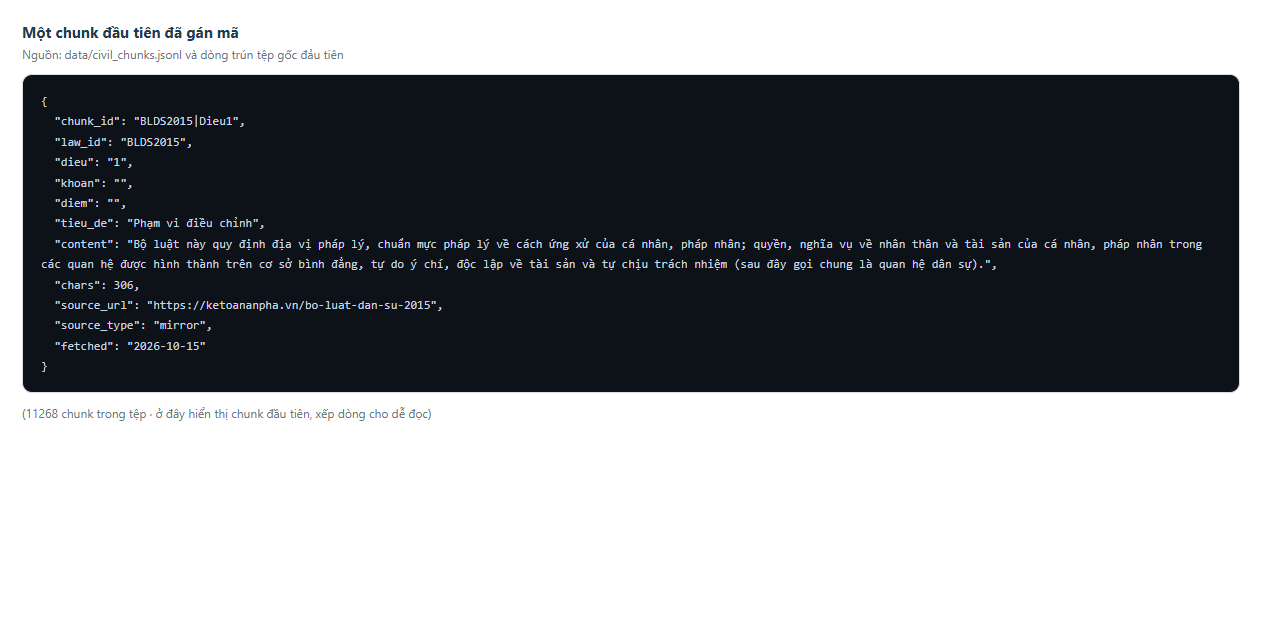
\includegraphics[width=\textwidth]{fig03_chunk_sample.png}
\caption{Chunk đầu tiên trong tệp \texttt{data/civil\_chunks.jsonl}. Nội dung lấy nguyên văn từ
tệp gốc trong kho, chỉ xếp lại thụt lề cho dễ đọc.}
\label{fig:chunk}
\end{figure}

\begin{table}[htbp]
\centering\small
\caption{Các trường của một chunk.}
\label{tab:chunkfields}
\begin{tabular}{@{}llp{8.6cm}@{}}
\toprule
\textbf{Trường} & \textbf{Ví dụ} & \textbf{Ý nghĩa} \\
\midrule
\texttt{chunk\_id} & \texttt{BLDS2015|Dieu1} & Mã duy nhất của chunk \\
\texttt{law\_id} & \texttt{BLDS2015} & Mã của văn bản chứa chunk \\
\texttt{dieu}, \texttt{khoan}, \texttt{diem} & \texttt{"27"}, \texttt{"1"}, \texttt{"a"} & Vị trí trong cấu trúc luật \\
\texttt{tieu\_de} & Phạm vi điều chỉnh & Tiêu đề của đoạn \\
\texttt{content} & (văn bản) & Nội dung đoạn \\
\texttt{chars} & \texttt{306} & Độ dài đoạn \\
\texttt{source\_url} & ketoananpha.vn/... & Nơi lấy nội dung \\
\texttt{source\_type} & \texttt{mirror} & Loại nguồn \\
\texttt{fetched} & \texttt{2026-10-15} & Ngày lấy \\
\bottomrule
\end{tabular}
\end{table}

Ba lý do mã phải bám theo cấu trúc pháp lý: (i) \emph{ổn định} --- nếu mã đổi sau mỗi lần chạy lại,
toàn bộ 11.267 vector và mọi cạnh dẫn chiếu đã tính phải làm lại; (ii) \emph{trích dẫn chính xác}
--- giữ nguyên ranh giới Điểm a/b/c giúp trích đủ ý, không thiếu không thừa; (iii) \emph{chia sẻ được}
--- người khác dùng chung mã này để nối vào tập dữ liệu của họ mà không phải chia lại dữ liệu.

% ============================== 4 ==============================
\section{Ba nơi lưu trữ trên cùng một bộ dữ liệu}

Cùng 11.267 chunk được lập chỉ mục theo ba cách để tra cứu khác nhau.

\begin{figure}[htbp]
\centering
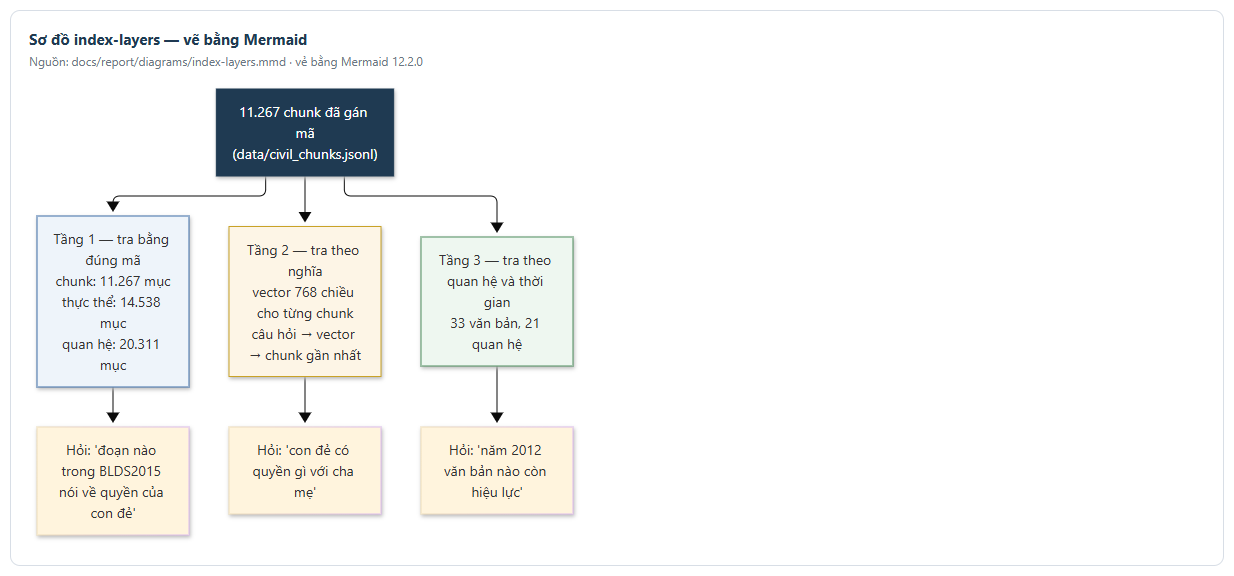
\includegraphics[width=\textwidth]{fig04_ba-tang-luu-tru.png}
\caption{Sơ đồ ba tầng lưu trữ. Vẽ bằng Mermaid; mã nguồn tại
\texttt{docs/report/diagrams/index-layers.mmd}.}
\label{fig:layers}
\end{figure}

\begin{table}[htbp]
\centering\small
\caption{Ba tầng chỉ mục trên cùng một bộ dữ liệu.}
\label{tab:layers}
\begin{tabular}{@{}cp{2.6cm}p{5.1cm}p{4.0cm}@{}}
\toprule
\textbf{Tầng} & \textbf{Số mục} & \textbf{Lưu gì} & \textbf{Dùng để làm gì} \\
\midrule
1 & 11.267 / 14.538 / 20.311 & Tra theo mã chunk, theo tên thực thể, theo quan hệ & Tra chính xác: đoạn nào, tên gì \\
2 & 11.267 vector 768 chiều & Mã hoá của từng chunk & Tra nghĩa: câu hỏi $\rightarrow$ chunk gần nhất \\
3 & 33 luật, 21 quan hệ & Đồ thị tri thức có chiều thời gian & Tra theo quan hệ và theo thời điểm \\
\bottomrule
\end{tabular}
\end{table}

Điểm cần nói thẳng: đây là JSON kèm kho vectơ phẳng, chưa phải cơ sở dữ liệu quan hệ đầy đủ
(xem mục \ref{sec:kho}).

% ============================== 5 ==============================
\section{Đồ thị tri thức}

Đồ thị chứa các văn bản luật (33 nút) và các quan hệ giữa chúng (21 cạnh). Mỗi nút mang
khoảng hiệu lực, số hiệu văn bản, số chunk và số lần được dẫn chiếu.

\begin{figure}[htbp]
\centering
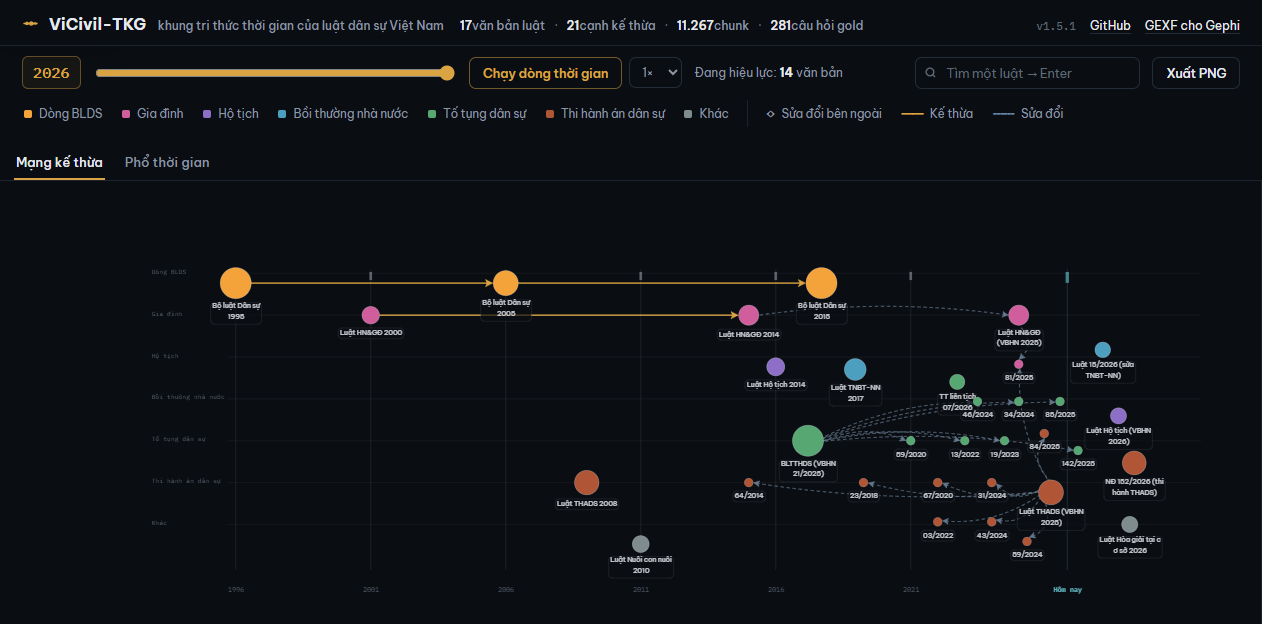
\includegraphics[width=\textwidth]{fig05_graph_2026.png}
\caption{Trạng thái đồ thị tại năm 2026: 14 văn bản còn hiệu lực, các luật đã hết hiệu lực được làm mờ.}
\label{fig:g2026}
\end{figure}

\begin{table}[htbp]
\centering\small
\caption{Các loại quan hệ trong đồ thị.}
\label{tab:relations}
\begin{tabular}{@{}lrl@{}}
\toprule
\textbf{Quan hệ} & \textbf{Số cạnh} & \textbf{Nghĩa} \\
\midrule
REPLACES & 3 & Luật mới thay thế luật cũ \\
AMENDS & 17 & Sửa đổi điều khoản cụ thể \\
CONSOLIDATES & 1 & Hợp nhất \\
\bottomrule
\end{tabular}
\end{table}

Quan hệ sửa đổi chỉ được nhận khi đọc được từ lời nói đầu của văn bản hợp nhất, không tin
vào đoạn trích từ công cụ tìm kiếm. Có một lần tin đoạn tìm kiếm đã tạo ra 142 cạnh sai; sau đó
toàn bộ quan hệ được dựng lại từ văn bản gốc.

% ============================== 6 ==============================
\section{Cập nhật theo đồ thị động và theo thời gian}

Đồ thị này có chiều thời gian. Kéo thanh thời gian là toàn bộ đồ thị tính lại trạng thái, chứ
không phải hai bản vẽ khác nhau.

\begin{figure}[htbp]
\centering
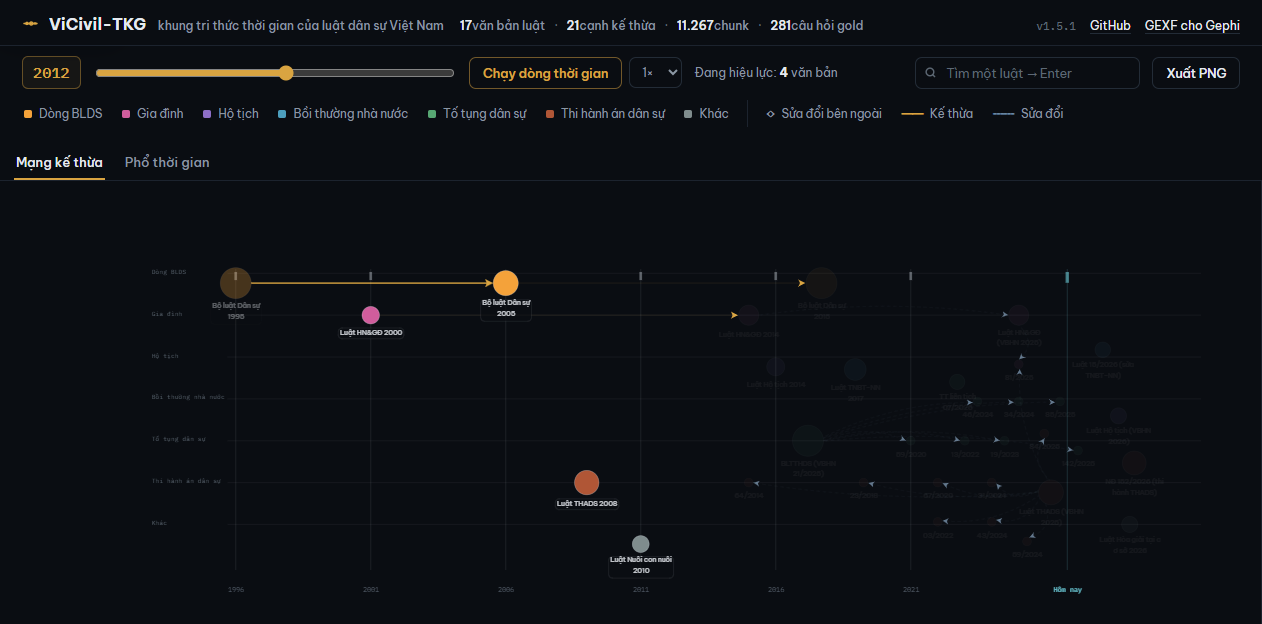
\includegraphics[width=\textwidth]{fig06_graph_2012.png}
\caption{Cùng đồ thị, tại thời điểm năm 2012: chỉ 4 văn bản còn hiệu lực, các luật chưa tới
hạn bị làm mờ.}
\label{fig:g2012}
\end{figure}

\begin{table}[htbp]
\centering\small
\caption{Kết quả truy vấn ``tại thời điểm T, luật nào còn hiệu lực''.}
\label{tab:temporal}
\begin{tabular}{@{}llp{9.6cm}@{}}
\toprule
\textbf{Mốc thời gian} & \textbf{Số luật còn hiệu lực} & \textbf{Kiểm tra tự động trong dữ liệu} \\
\midrule
2000-01-01 & 1 & Chỉ Bộ luật Dân sự 1995 \\
2010-06-01 & 1 & Chỉ Bộ luật Dân sự 2005 \\
2020-06-01 & 2 & Bộ luật Dân sự 2015 và Luật Hôn nhân và Gia đình 2014 \\
2026 & 14 & Trạng thái hiện tại của trang xem \\
\bottomrule
\end{tabular}
\end{table}

% ============================== 7 ==============================
\section{Trình xem}

Trang xem có hai phần. Phần \emph{Mạng kế thừa} vẽ bằng thư viện AntV G6, có thanh thời gian,
tìm kiếm theo tên, khung chi tiết và nút xuất ảnh PNG. Phần \emph{Phổ thời gian} vẽ bằng Vega-Lite
từ một tệp spec công khai, ai cũng dùng lại được.

\begin{figure}[htbp]
\centering
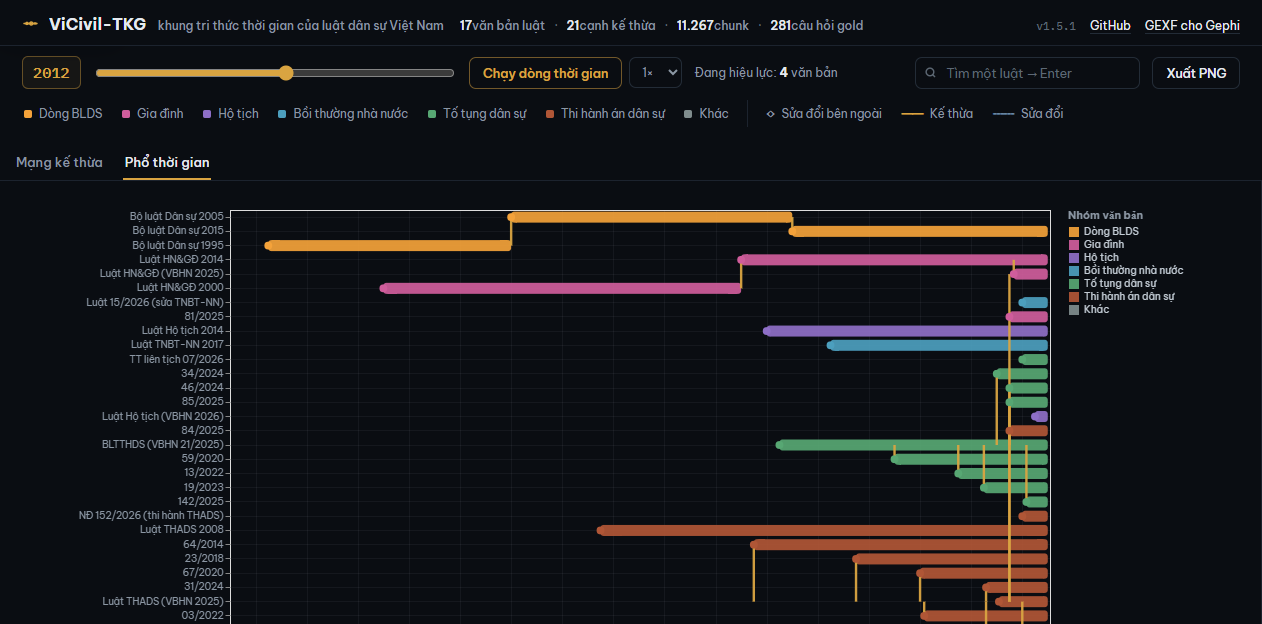
\includegraphics[width=\textwidth]{fig07_timeline_tab.png}
\caption{Phổ thời gian: dải thời gian hiệu lực của từng văn bản, dựng bằng Vega-Lite từ tệp
spec \texttt{law\_timeline.vl.json} có trong kho.}
\label{fig:timeline}
\end{figure}

\begin{figure}[htbp]
\centering
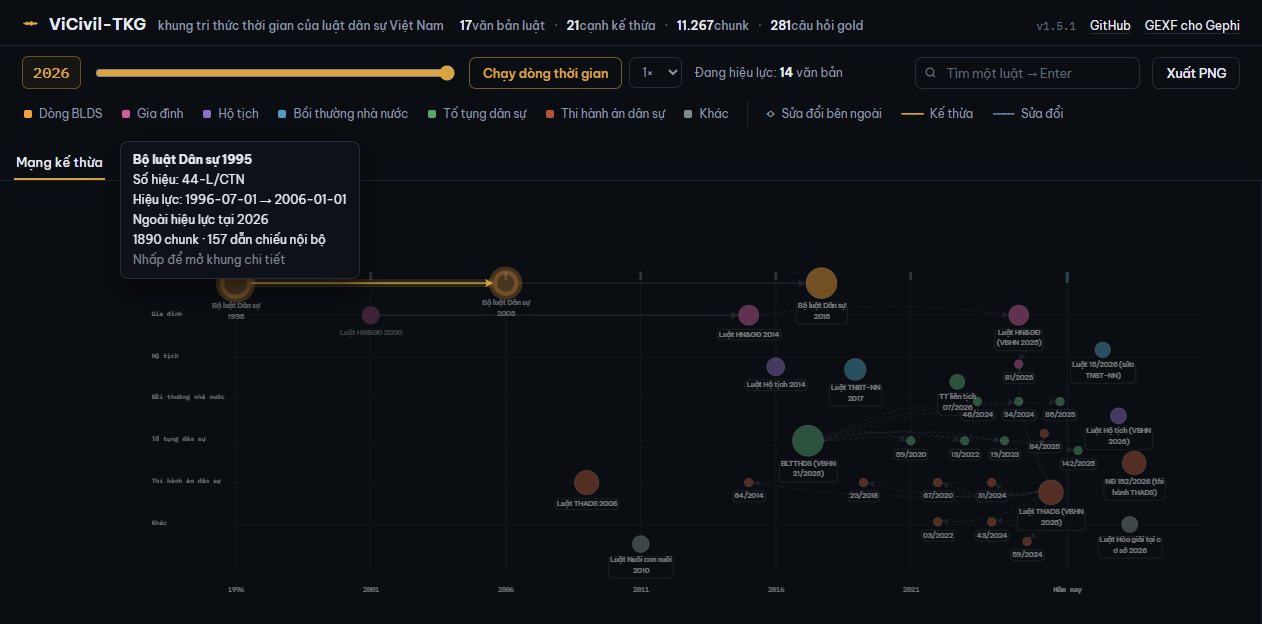
\includegraphics[width=\textwidth]{fig08_tooltip.png}
\caption{Rê chuột vào một luật: số hiệu, khoảng hiệu lực, số chunk và số lần dẫn chiếu;
đồng thời chuỗi kế thừa của luật đó được làm sáng, các phần tử khác mờ đi.}
\label{fig:tooltip}
\end{figure}

\begin{figure}[htbp]
\centering
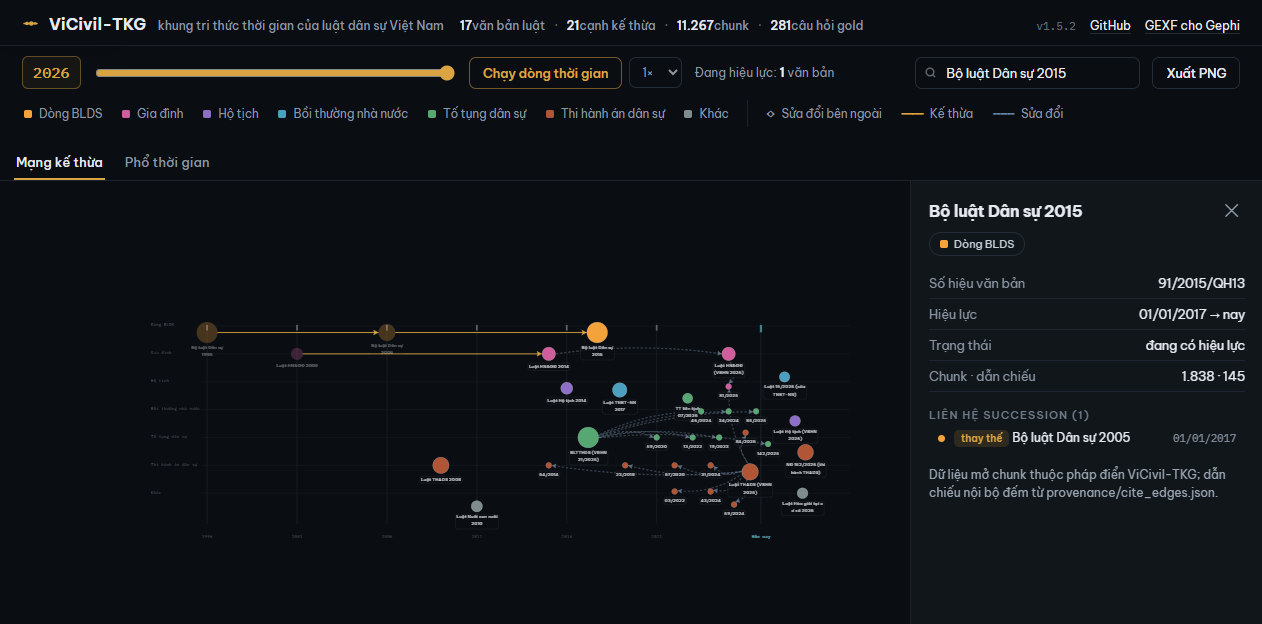
\includegraphics[width=\textwidth]{fig09_drawer.png}
\caption{Khung chi tiết: ví dụ Bộ luật Dân sự 2015 --- số hiệu 91/2015/QH13, có hiệu lực từ
01/01/2017 đến nay, 1.838 chunk, 145 lần dẫn chiếu, và quan hệ thay thế với Bộ luật Dân sự 2005.}
\label{fig:drawer}
\end{figure}

Trang xem được viết thành một tệp HTML duy nhất, nhúng sẵn cả bốn thư viện, nên chạy được khi
mất mạng và mở trực tiếp từ ổ đĩa.

% ============================== 8 ==============================
\section{Thử nghiệm}

\begin{figure}[htbp]
\centering
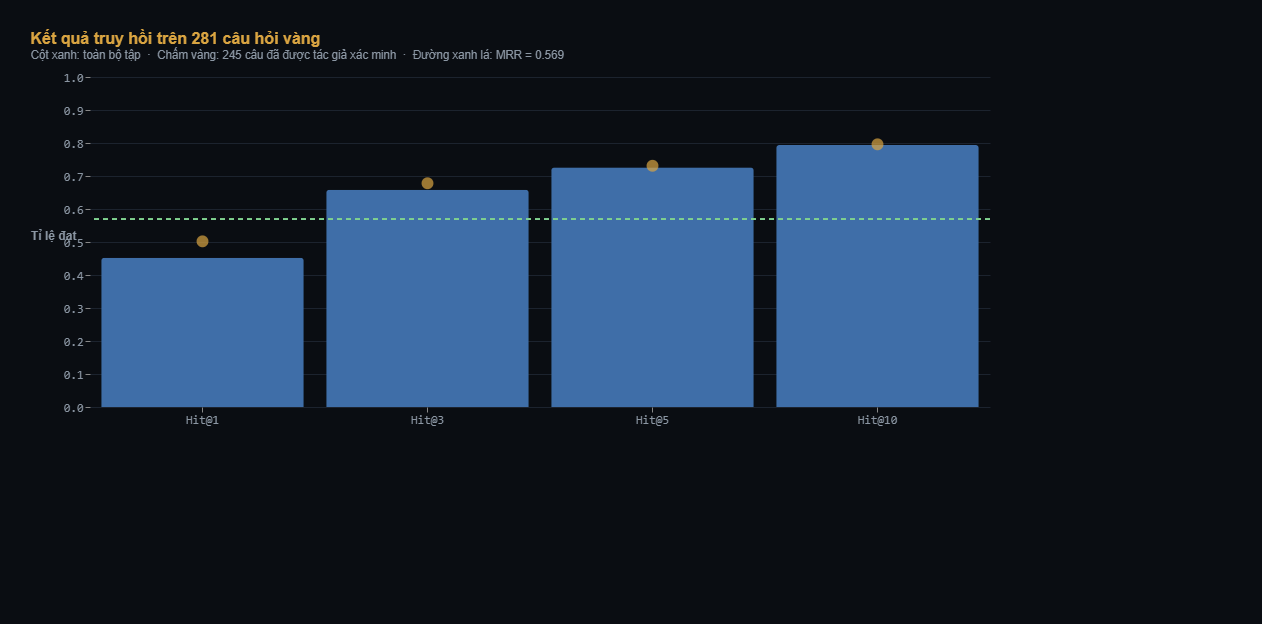
\includegraphics[width=0.92\textwidth]{fig10_eval.png}
\caption{Kết quả truy hồi trên 281 câu hỏi có đáp án. Biểu đồ vẽ bằng Vega-Lite từ đúng tệp
kết quả \texttt{benchmark/law\_eval\_v12.json}.}
\label{fig:eval}
\end{figure}

Bộ kiểm tra gồm 281 câu hỏi; ngày hỏi phải nằm trong khoảng hiệu lực của văn bản chứa đáp án.

\begin{table}[htbp]
\centering\small
\caption{Kết quả truy hồi theo hai cách chia tập câu hỏi.}
\label{tab:eval}
\begin{tabular}{@{}lcc@{}}
\toprule
\textbf{Chỉ số} & \textbf{Toàn bộ 281 câu} & \textbf{245 câu đã được tác giả xác minh} \\
\midrule
Tìm đúng ở lần 1 (Hit@1) & 0,452 & 0,502 \\
Tìm đúng trong 3 lần (Hit@3) & 0,658 & 0,678 \\
Tìm đúng trong 5 lần (Hit@5) & 0,726 & 0,731 \\
Tìm đúng trong 10 lần (Hit@10) & 0,794 & 0,796 \\
Độ tin cậy tổng hợp (MRR) & 0,569 & --- \\
\bottomrule
\end{tabular}
\end{table}

Điểm đáng nói thẳng: 32 câu thuộc nhóm ``đáp án đúng nhưng hệ thống trả về nguồn khác'' chỉ đạt
Hit@1 = 0,062, kéo số trung bình toàn bộ xuống. Đây là hạn chế của \emph{thang đo}, chưa chắc là
hạn chế của hệ thống. Vì vậy báo cáo này lấy số trên tập 245 câu đã xác minh làm con số chính,
nhóm còn lại để riêng.

% ============================== 9 ==============================
\section{Phân bố dữ liệu}

\begin{figure}[htbp]
\centering
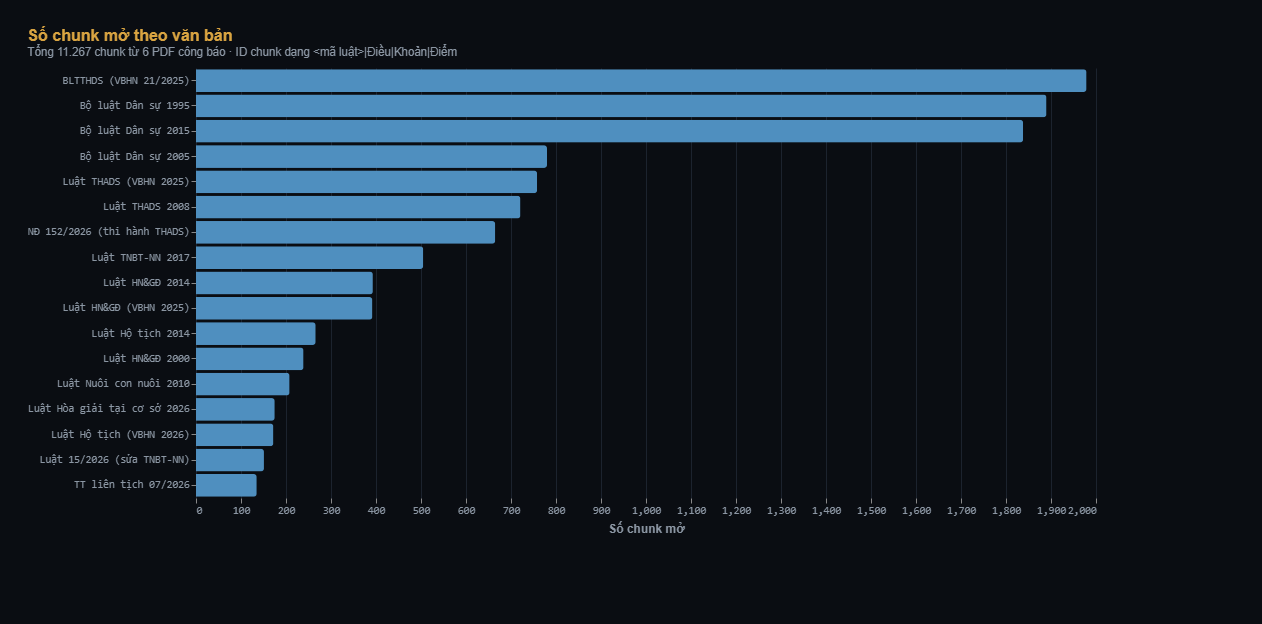
\includegraphics[width=0.95\textwidth]{fig11_chunk_distribution.png}
\caption{Số chunk mở theo từng văn bản. Biểu đồ vẽ bằng Vega-Lite từ đúng tệp
\texttt{data/civil\_chunks.jsonl}.}
\label{fig:dist}
\end{figure}

Bốn văn bản chiếm hơn một nửa số chunk. Do đó không thể dùng một quy tắc cắt chunk duy nhất cho
toàn bộ kho; các luật chuyên ngành có cấu trúc và độ dài đoạn khác hẳn bộ luật dân sự.

% ============================== 10 ==============================
\section{Chia sẻ cho người khác}

\begin{figure}[htbp]
\centering
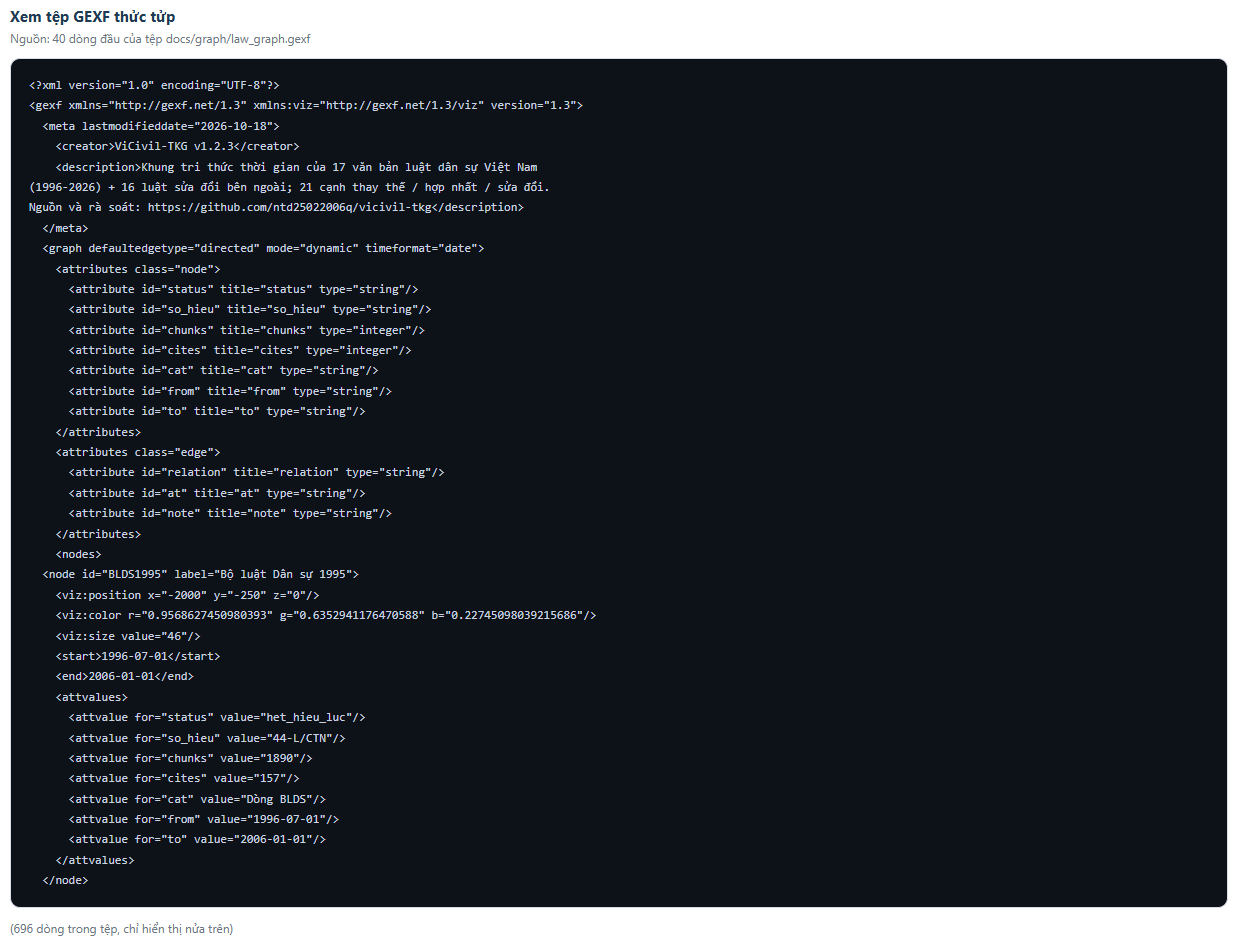
\includegraphics[width=\textwidth]{fig12_gexf.png}
\caption{40 dòng đầu của tệp \texttt{docs/graph/law\_graph.gexf} (tệp có 696 dòng).
Ảnh chụp nguyên văn từ tệp gốc trong kho.}
\label{fig:gexf}
\end{figure}

Đồ thị được xuất ra định dạng GEXF 1.3 ở chế độ \textit{dynamic}, nên khi mở bằng Gephi hoặc
Gephi-Lite, người nhận có được đồ thị kèm trục thời gian và mọi thuộc tính (số hiệu, số chunk,
số lần dẫn chiếu). Phần chưa làm: chưa xuất định dạng RDF/JSON-LD để nạp vào kho tri thức chuẩn,
và chưa cấp mã DOI cho từng phiên bản.

% ============================== 11 ==============================
\section*{Khó khăn gặp phải và đề xuất cải tiến}
\label{sec:kho}
\addcontentsline{toc}{section}{Khó khăn gặp phải và đề xuất cải tiến}

\begin{table}[htbp]
\centering\small
\caption{Những khó khăn đã gặp và cách xử lý.}
\label{tab:issues}
\begin{tabular}{@{}p{6.0cm}p{5.4cm}p{4.4cm}@{}}
\toprule
\textbf{Khó khăn} & \textbf{Biểu hiện} & \textbf{Đã xử lý thế nào} \\
\midrule
Tin đoạn trích tìm kiếm làm nhiễu quan hệ & 142 cạnh sửa đổi sai & Chỉ nhận quan hệ từ lời nói đầu văn bản hợp nhất \\
Ngày hỏi nằm ngoài thời gian hiệu lực & 48 câu hỏi không dùng được & Kiểm tra ngày hỏi trước khi nhận câu \\
Ghi đè làm mất dữ liệu đã trích & mất khoảng 2.900 dòng & Bắt buộc sao lưu trước khi ghi đè \\
Hệ thống trả nguồn khác với đáp án đúng & 32 câu chỉ đạt 0,062 & Công bố đúng số thay vì làm đẹp con số \\
PDF ảnh không có lớp chữ & không tách được chunk & Tách riêng hàng chờ đọc lại (OCR), không đoán \\
Thư viện vẽ chạy sai trên một số trình duyệt & trang trắng, không báo lỗi & Chạy thử trên Chrome và Edge thật trước khi phát hành \\
\bottomrule
\end{tabular}
\end{table}

\textbf{Đề xuất làm tiếp, theo thứ tự giá trị:}
\begin{enumerate}
\item Xuất định dạng RDF/JSON-LD để nạp vào kho tri thức chuẩn (Neo4j, rdf4j). Cấu trúc quan hệ
đã sẵn có nên công việc này không tốn nhiều.
\item Đưa đoạn văn bản lên đồ thị (nút cấp Điều/Khoản nối vào luật) để trả lời trực tiếp câu hỏi
kiểu ``điều nào bị sửa, sửa những gì''.
\item Sửa thang đo: chấp nhận nhiều đáp án đúng về mặt pháp lý, và dùng một mô hình ngôn ngữ lớn
làm người chấm cho nhóm câu có nguồn khác.
\item Khi có văn bản mới, chỉ tính toán phần mới (chunk và vector của phần mới) thay vì chạy lại toàn bộ.
\item Bổ sung văn bản chưa số hóa: 4 câu hỏi chưa đạt trọn vẹn có liên quan đến vấn đề này.
\end{enumerate}

% ============================== 12 ==============================
\section{Kiểm tra lại trước khi phát hành}

\begin{table}[htbp]
\centering\small
\caption{Các kiểm tra thực hiện trước khi phát hành.}
\label{tab:checks}
\begin{tabular}{@{}p{7.2cm}p{8.4cm}@{}}
\toprule
\textbf{Kiểm tra} & \textbf{Kết quả} \\
\midrule
Mã SHA-256 của mọi tệp & 62/62 khớp; hai gương giống nhau (trừ README vì chính sách khác nhau) \\
Quét chữ ẩn, khoá bí mật & Không phát hiện \\
Mọi tệp JSON/JSONL/GEXF mở được & Có \\
Chạy trên Chrome thật và Edge thật & Không có lỗi JavaScript \\
Trang xem chạy khi mất mạng & Có (không cần CDN) \\
Truy vấn thời gian tự kiểm & Đúng ở cả 3 mốc 2000, 2010, 2020 \\
\bottomrule
\end{tabular}
\end{table}

% ============================== PHỤ LỤC ==============================
\clearpage
\appendix
\section{Bản đồ yêu cầu}

\begin{table}[htbp]
\centering\small
\caption{Đối chiếu từng yêu cầu với phần tương ứng trong báo cáo.}
\label{tab:reqmap}
\begin{tabular}{@{}p{6.4cm}p{1.4cm}p{8.0cm}@{}}
\toprule
\textbf{Yêu cầu} & \textbf{Mục} & \textbf{Kết quả} \\
\midrule
Chia file bộ luật thành các chunk & \ref{sec:kho} & 11.267 chunk theo Điều/Khoản/Điểm, mã ổn định \\
Lưu trữ thành cơ sở dữ liệu các chunk có nhãn & \ref{tab:layers} & 3 tầng chỉ mục: tra theo mã, tra theo nghĩa, tra theo quan hệ \\
Chia sẻ chunk và node & \ref{fig:gexf} & GEXF 1.3 mở bằng Gephi, mã chunk dùng chung được --- còn thiếu RDF và DOI \\
Xây dựng đồ thị tri thức theo cách người ta làm & \ref{tab:relations} & 33 nút, 21 cạnh có nhãn và mốc thời gian --- nút mới ở cấp luật \\
Cập nhật hướng theo đồ thị động & \ref{fig:g2012} & Thanh thời gian: 2012 có 4 luật, 2026 có 14 luật \\
Cập nhật thời gian & \ref{tab:temporal} & Mỗi luật có khoảng hiệu lực; tự kiểm ở 3 mốc thời gian \\
Nêu khó khăn và đề xuất cải tiến & \ref{sec:kho} & 6 khó khăn, 5 đề xuất cụ thể \\
\bottomrule
\end{tabular}
\end{table}

\section{Cách làm ra từng hình}

\begin{table}[htbp]
\centering\small
\caption{Công cụ và nguồn của từng hình trong báo cáo.}
\label{tab:figsrc}
\begin{tabular}{@{}clp{4.4cm}p{5.4cm}@{}}
\toprule
\textbf{Hình} & \textbf{Nội dung} & \textbf{Công cụ} & \textbf{Nguồn} \\
\midrule
\ref{fig:pipeline} & Quy trình A $\rightarrow$ Z & Mermaid 12.2.0 & \texttt{docs/report/diagrams/pipeline.mmd} \\
\ref{fig:chunk} & 14 chunk đầu tiên & Chụp từ trình duyệt & \texttt{data/civil\_chunks.jsonl} \\
\ref{fig:layers} & Ba tầng lưu trữ & Mermaid 12.2.0 & \texttt{docs/report/diagrams/index-layers.mmd} \\
\ref{fig:g2026} & Đồ thị năm 2026 & Chụp từ trình duyệt & \texttt{docs/graph/explorer.html} \\
\ref{fig:g2012} & Đồ thị năm 2012 & Chụp từ trình duyệt & \texttt{docs/graph/explorer.html} \\
\ref{fig:timeline} & Phổ thời gian & Chụp từ trình duyệt & \texttt{docs/graph/explorer.html} \\
\ref{fig:tooltip} & Thẻ tin khi rê chuột & Chụp từ trình duyệt & \texttt{docs/graph/explorer.html} \\
\ref{fig:drawer} & Khung chi tiết & Chụp từ trình duyệt & \texttt{docs/graph/explorer.html} \\
\ref{fig:eval} & Kết quả truy hồi & Vega-Lite 5.21.0 & \texttt{benchmark/law\_eval\_v12.json} \\
\ref{fig:dist} & Chunk theo văn bản & Vega-Lite 5.21.0 & \texttt{data/civil\_chunks.jsonl} \\
\ref{fig:gexf} & 40 dòng đầu tệp GEXF & Chụp từ trình duyệt & \texttt{docs/graph/law\_graph.gexf} \\
\bottomrule
\end{tabular}
\end{table}

\section{Các thành phần dùng trong báo cáo}

\begin{itemize}
\item \textbf{AntV G6 5.1.1} (MIT) --- vẽ đồ thị kế thừa.
\item \textbf{Vega-Lite 5.21.0} và \textbf{Vega 5.30.0} (BSD-3-Clause) --- vẽ phổ thời gian và các biểu đồ.
\item \textbf{vega-embed 6.26.0} (BSD-3-Clause) --- nhúng biểu đồ Vega-Lite vào trang.
\item \textbf{Mermaid 12.2.0} (MIT) --- vẽ hai sơ đồ trong báo cáo này.
\item \textbf{GEXF 1.3} --- định dạng trao đổi đồ thị mở của Gephi.
\item \textbf{MiKTeX / XeLaTeX} --- dàn trang báo cáo này.
\end{itemize}

\begin{thebibliography}{9}
\bibitem{g6} AntV G6 5.1.1 (MIT). \texttt{github.com/antvis/G6}.
\bibitem{vega} Vega 5.30.0, Vega-Lite 5.21.0, vega-embed 6.26.0 (BSD-3-Clause).
\texttt{github.com/vega}.
\bibitem{gexf} GEXF 1.3 --- định dạng đồ thị mở của Gephi. \texttt{gexf.net}.
\bibitem{mermaid} Mermaid 12.2.0 (MIT). \texttt{mermaid.js.org}.
\bibitem{repo} Kho dữ liệu ViCivil-TKG v1.5.4. \texttt{github.com/ntd25022006q/vicivil-tkg}.
\end{thebibliography}

\end{document}